\documentclass[lettersize,journal]{IEEEtran}
\usepackage{amsmath,amsfonts}
\usepackage[french]{babel}
\usepackage[justification=centering]{caption}
\usepackage{algorithmic}
\usepackage{algorithm}
\usepackage{array}
\usepackage[caption=false,font=normalsize,labelfont=sf,textfont=sf]{subfig}
\usepackage{textcomp}
\usepackage{stfloats}
\usepackage{url}
\usepackage{verbatim}
\usepackage{graphicx}
\usepackage{cite}
\hyphenation{op-tical net-works semi-conduc-tor IEEE-Xplore}
% updated with editorial comments 8/9/2021

\begin{document}

\title{A Sample Article Using IEEEtran.cls\\ for IEEE Journals and Transactions}

\author{Wei Teng, Nan Lin, Yu'ang Ding, Qingyue Deng, Ke Ma, Bingru Wang}

% The paper headers
\markboth{Journal of \LaTeX\ Class Files,~Vol.~14, No.~8, August~2021}%
{Shell \MakeLowercase{\textit{et al.}}: A Sample Article Using IEEEtran.cls for IEEE Journals}

\IEEEpubid{}
% Remember, if you use this you must call \IEEEpubidadjcol in the second
% column for its text to clear the IEEEpubid mark.

\maketitle

\begin{abstract}
This document déscribes the most common article elements and how to use the IEEEtran class with \LaTeX \ to produce files that are suitable for submission to the IEEE.  IEEEtran can produce conference, journal, and technical note (correspondence) papers with a suitable choice of class options. 
\end{abstract}

\begin{IEEEkeywords}
Article submission, IEEE, IEEEtran, journal, \LaTeX, paper, template, typesetting.
\end{IEEEkeywords}

\section{Introduction}
\IEEEPARstart{A}{vec} une attention croissante portée aux énergies propres et à la mobilité durable, les véhicules électriques émergent rapidement en tant que mode de transport respectueux de l'environnement et efficace. Dans cette tendance ascendante, les courses de voitures électriques gagnent en popularité en tant que nouveau domaine compétitif. Comparées aux véhicules à moteur à combustion interne traditionnels, les voitures électriques présentent des avantages uniques dans leurs systèmes de propulsion et leur utilisation de l'énergie, grâce notamment aux systèmes de récupération d'énergie au freinage (BERS/RBS), prolongeant ainsi l'autonomie des véhicules. Cependant, maximiser ces avantages pour obtenir des performances optimales reste un défi lors des courses de vitesse.\par
Le système de récupération d'énergie au freinage des voitures électriques est une technologie courante visant à améliorer l'efficacité énergétique de ces véhicules. Lorsque les voitures électriques freinent, le système de freinage convertit l'énergie cinétique générée par l'inertie des roues en énergie électrique, puis la stocke dans la batterie. Ainsi, l'énergie produite lors du ralentissement et de l'arrêt du véhicule n'est pas gaspillée mais récupérée pour recharger la batterie, prolongeant ainsi la distance parcourue par le véhicule.\par

Les courses de voitures électriques, en tant que discipline sportive extrêmement exigeante, comprennent généralement diverses épreuves telles que des épreuves d'accélération, de montée, de virages, etc., chacune imposant des exigences différentes en termes de performances des véhicules. Cela nécessite que les voitures électriques atteignent leur meilleur niveau dans chaque épreuve, avec une répartition optimale de la puissance par le pilote, c'est-à-dire en accélérant et en freinant au moment opportun.
Le système de récupération d'énergie au freinage, en tant que caractéristique clé des voitures électriques, offre une opportunité unique de récupérer l'énergie pendant les phases de ralentissement et de freinage, améliorant ainsi l'autonomie et les performances globales des véhicules. Par conséquent, en optimisant la répartition de la puissance du système de récupération d'énergie au freinage, nous pouvons améliorer davantage la compétitivité des voitures électriques dans les courses de vitesse et stimuler le développement de la technologie des voitures électriques.\par
Ce document présentera le contexte et l'importance des courses de voitures électriques, discutera des modèles de puissance critique existants et proposera une solution d'optimisation de la répartition de la puissance des voitures électriques sur les circuits de course. Nous croyons que cette recherche apportera de nouvelles perspectives et méthodes pour les stratégies de compétition dans les courses de voitures électriques et contribuera à l'avancement et à l'application de la technologie des voitures électriques.


\section{Préparation du modèle}
\subsection{Hypothèses et explications}

\subsection{Notations}

\begin{table}[H]
    \centering
    \begin{tabular}{c|c|c|c}
    \hline
       Symbole  & Description &  Symbole  & Description  \\
        \hline
        W & énergie totale & $P_{con}$  & puissance consommée  \\
         
        $P_{rec}$ & puissance récupérée & PC &  puissance critique\\

         VC& vitesse critique & $\rho$  & densité de l'air\\

         $C_d$& coefficient de résistance  & A &  surface de stress \\

         $\mu$& coefficient de la friction & T & moment de torsion \\

         $\omega$& vitesse angulaire & v & vitesse  \\

         u & puissance du moteur & s & distance  \\
       
         $\theta$ &Inclinaison de la pente &  & \\
         \hline
    \end{tabular}
\caption{Notations}
\label{tab:my_label}
\end{table}

\section{Le modèle de puissance critique}

\subsection{Le modèle de récupération d'énergie}
Supposons que la voiture consomme de l’énergie en roulant, mais qu’elle en récupère également une partie. Cependant, lorsque la vitesse de la voiture est suffisamment élevée, l’énergie consommée est bien supérieure à l’énergie qui peut être récupérée, et l’énergie globale montre une tendance de consommation. Au contraire, lorsque la vitesse de la voiture est faible, l’énergie récupérée est supérieure à l’énergie consommée, et l’énergie globale montre une tendance à la hausse.\par

Entre les deux, il existe une vitesse critique (\textbf{VC}) et une puissance critique (\textbf{PC}) associée telles que la puissance consommée est égale à la puissance récupérée lorsque le moteur ne fonctionne pas.\\
\begin{equation}
    \frac{dW}{dt} = P_{rec} - P_{con}
\end{equation}
où W est l'énergie totale et $P_{con} > 0$ et $P_{rev} > 0$ sont les énergies consumées et récupérées respectivement.
Ici, nous ne prenons en compte que la puissance consommée par la résistance, et non la puissance consommée par le moteur lui-même.

\subsection{Détermination des paramètres importants}
Afin de déterminer les valeurs de PC et de VC, nous devons connaître les courbes de relation entre $P_{con}$, $P_{rec}$ et la vitesse de la voiture $v$.\par
Supposons que dans le processus de conduite d'un véhicule électrique, il existe deux résistances, la friction et la résistance à l'air:
\begin{equation}
    \begin{cases}
        F_r = \frac{1}{2} \rho C_{d} A v^{2} \\
        F_f = \mu mg
    \end{cases}
\end{equation}
avec $\rho$ la densité de l'air, $C_d$ le coefficient de résistance à l'air, $A$ la surface de stress et $\mu$ le coefficient de la friction.\par
Donc la puissance consomée doit neutraliser les puissances de la résistance, c'est-à-dire,
\begin{equation}
    P_{con} = \frac{1}{3600 \eta}(\mu mg + \frac{1}{2} \rho C_{d} A v^{2}) \cdot v
\end{equation}
avec $\eta$ l'efficacité de la moteur.\par

De plus, Nous utilisons la relation entre le moment de torsion et la vitesse angulaire:
\begin{equation}
    \begin{cases}
        P= &T \times \omega + b \\
        v= &\omega \times r
    \end{cases}
\end{equation}
avec $T$ le moment de torsion , $r$ le rayon du pneu et $b$ un constant qui représente la puissance alimentée comme par exemple des panneaux solaires. \par

\begin{table}[H]
    \centering
    \begin{tabular}{c|c|c|c|c|c}
    
    \hline
         m(kg)& 18000 & g($m\dot s^{-2}$ & 9.8 & $\mu$ & 0.016 \\
    \hline
         A($m^{2}$)& 8.16 & $C_d$ & 0.6 & $\eta$  & 0.86\\
         \hline
    \end{tabular}
    \caption{Paramètres}
    \label{tab:my_label}
\end{table}

D'après le tableau ci-dessus, nous pouvons obtenir les deux courbes suivantes:
\begin{figure}[H]
\centering
 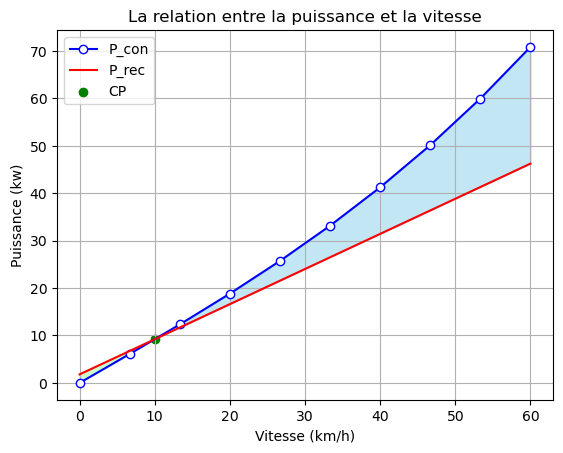
\includegraphics[width=0.7\linewidth]{CP.png}
\caption{Les puissances consommée et récupérée}
\end{figure}
Ensuite nous calculons les coordonnées de leur intersection.
\begin{equation}
    \begin{cases}
        PC = 9.27 \text{Kw} \\
        VC = 10.08 km /h
    \end{cases}
\end{equation}
Il faut noter que ces paramètres ne sont qu'un résultat approximatif, les paramètres plus précis doivent être obtenus par des méthodes plus sérieuses avec de nombreux expériments.


\section{Formule de contrôle optimale}
Dans cette partie, nous construisons principalement le modèle d’optimisation de la course de véhicules électriques et proposons le problème d’optimisation que nous voulons résoudre.\par
Lors de la conduite d’un véhicule électrique, l’ensemble du système peut être considéré comme ayant trois états :
\begin{itemize}
    \item La distance parcourue $s$
    \item La vitesse du véhicule $v$
    \item L’énergie totale d’un véhicule électrique $W$
\end{itemize}\par
De plus le système a une seule entrée $u$ qui est la puissance du véhicule. Notons x le vecteur d'état, alors nous avons la propriété suivante:
\begin{equation}
    \dot{x} = f(x(t), u(t)) = [f_1\ f_2\ f_3]^{T}
\end{equation}
où
\begin{equation}
    x = [s(t)\ v(t)\ W(t)]^{T}
\end{equation}
avec f la fonction qui relie le changement d'état avec l'état lui-même et l'entrée. Analysons ces trois grandeurs une par une et pour le permier état:
\begin{equation}
    \frac{ds}{dt} = v \overset{Not}{=} f_1
\end{equation}
Et pour le deuxième état nous utilisons la deuxième loi de Newton sur le véhicule. Au total, nous prenons en compte trois forces: la force motrice, la friction et la résistance à l'air.
\begin{equation}
    m\frac{dv(t)}{dt} = \frac{u(t)}{v(t)} - mg(\sin (\theta)+ \mu \cos (\theta))-\frac{1}{2}\rho C_{d}A v(t)^{2}
\end{equation}
où $\theta$ est l'inclinaison de la route, qui est positive pour un chemin montant et négative pour un chemin descendant.
\begin{figure}[H]
    \centering
    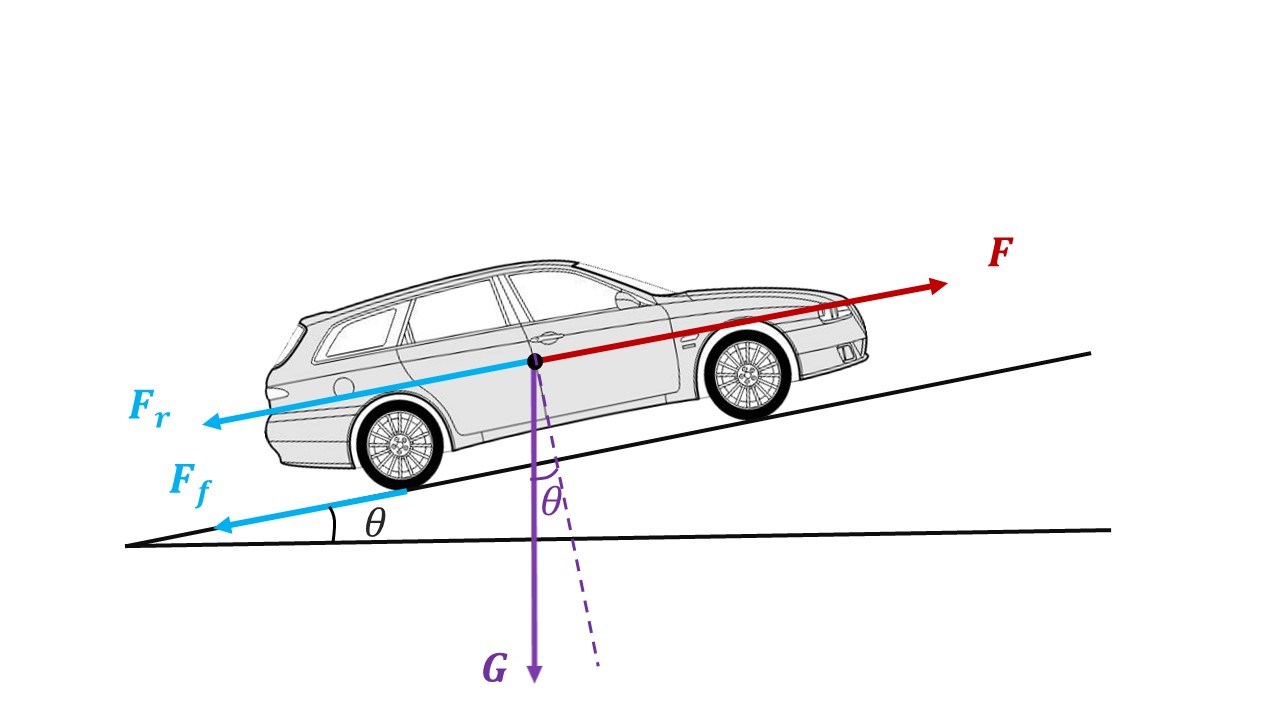
\includegraphics[width=1\linewidth]{force.jpg}
    \caption{Analyse des forces}
    \label{fig:enter-label}
\end{figure}

Donc nous pouvons obtenir que:
\begin{equation}
\begin{aligned}
    \frac{dv(t)}{dt} &= \frac{u(t)}{mv(t)} - g(\sin (\theta)+ \mu \cos (\theta))-\frac{1}{2m}\rho C_{d}A v(t)^{2}\\
    &\overset{Not}{=} f_2
\end{aligned}
\end{equation}
D'après l'équation 1 nous pouvons obtenir:
\begin{equation}
    \frac{dW}{dt} = P_{rec} - P_{con} \overset{Not}{=} f_3
\end{equation}
avec $u(t)$ la puissance consommée par le moteur.
Ensuite nous pouvons établir notre modèle d'optimisation comme:
\begin{equation}
    \underset{u(t)}{\min}\ \bf{J} = \int_{t_0}^{t_f} dt
\end{equation}
avec les contraintes suivantes:
\begin{itemize}
    \item modèle d'état : $\dot{x} = f(x(t), u(t))$
    \item limite de la vitesse: $0 \leq v(t) \leq v_{max}$
    \item limite de l'énergie totale :$0 \leq W(t) \leq W_{max}$
    \item limite de la puissance: $0 \leq u(t) \leq P_{max}(w,v)$
\end{itemize}

\section{Solutions}
\subsection{Les conditions nécessaires}
Dans cette partie nous utilisons Pontryagin’s Minimum Principle (PMP) pour trouver la solution optimale de ce problème. Nous voulons trouver une entrée $u$ qui minimise la fonction hamiltonienne sans constraintes:
\begin{equation}
    H(x(t),u(t),\lambda(t)) = L(x(t),u(t)) + \lambda^{T}(t)f
\end{equation}
où $\lambda = [\lambda_1, \lambda_2, \lambda_3]^{T}$ et $L$ est la fonction nous voulons minimiser (Dans ce cas c'est le temps).
Et puis nous ajoutons des contraintes sur cette fonction.\\
La contrainte sur la puissance peut s'écrire comme :
\begin{equation}
    C = u(t) - u_{max} \leq 0
\end{equation}
Donc la fonction Hamitolnienne est sous la forme:
\begin{equation}
    H = L + \lambda^{T}(t)f + \mu C
\end{equation}
avec
\begin{equation}
    \mu \begin{cases}
        \geq 0 \quad C=0\\
         = 0 \quad C < 0
    \end{cases}
\end{equation}
De plus, il y a des constraintes qui ne relient pas directement avec l'entrée $u$. On note S comme:
\begin{equation}
    S = \begin{bmatrix}
	v(t) - v_{max}  \\
    -v(t) \\
    W(t) - W_{max}\\
    -W(t)
\end{bmatrix} \leq \Vec{0}
\end{equation}
Lorsque les contraintes ne sont pas des fonctions de l’entrée de contrôle u, nous prennons des dérivées temporelles successives de S et remplaçons $\dot{v}$ et $\dot{w}$ par $f_2$ et $f_3$, respectivement, jusqu’à ce que nous obtenions une expression qui dépend explicitement de $u$. Donc nous obtenons:
\begin{equation}
    H = L + \lambda^{T}(t)f + \mu C + \eta^{T}S^{(1)}
\end{equation}
avec $\eta = [\eta_1,\eta_2,\eta_3,\eta_4]^{T}$ et
\begin{equation}
    \eta_{i}\begin{cases}
        \geq 0 \quad S_{i}^{(1)} = 0\\
         = 0 \quad S_{i}^{(1)} < 0
    \end{cases} for \quad i = 1,2,3,4
\end{equation}
En outre, la relation entre les paramètres $\lambda$ et H:
\begin{equation}
    \dot{\lambda}^{T} = -\frac{\partial H}{\partial x} = -\frac{\partial L}{\partial x} - \lambda^{T}\frac{\partial f}{\partial x} - \mu \frac{\partial C}{\partial x} - \eta^{T}\frac{\partial S}{\partial x}
\end{equation}
Par conséquent, 
\begin{equation}
    \begin{cases}
        \dot{\lambda_{1}} = \lambda_{2}g\theta'(s)(\cos(\theta(s)) - \mu \sin(\theta(s))\\
        \dot{\lambda_{2}} = -\lambda_1 + \frac{\lambda_2}{m} (\frac{u}{v^2}+C_{d}\rho A v)\\
        \dot{\lambda_{3}} = 0
    \end{cases}
\end{equation}
Une condition nécessaire à l’optimalité est que l’entrée de commande u, minimise le hamiltonien.
Donc nous calculons la dérivée de H par rapport à $u$ .
\begin{equation}
    \frac{\partial H}{\partial u } = \frac{\lambda_{2}}{mv}-\lambda_{3}+\frac{1}{mv}(\eta_1-\eta_2)+(\eta_4-\eta_3)+\mu
\end{equation}
\textbf{Case 1: $\mu > 0$} , c'est-à-dire $u = u_{max}$\\
\textbf{Case 2: $\eta_1$ et $\eta_2$ non tous nuls}. C'est-à-dire  $\dot{v} = 0$, donc on note la puissance $u_{\dot{v}=0}$.\\
\textbf{Case 3: $\eta_3$ et $\eta_4$ non tous nuls}.  C'est-à-dire $\dot{W} = 0$ donc $P_{rec} = P_{con}$ et u est maintenant égale à CP.\\
\textbf{Case 4: $\mu = \eta_1 = \eta_2 = \eta_3 = \eta_4 = 0 $}. C'est-à-dire 
\begin{equation}
    \frac{\partial H}{\partial u } = \frac{\lambda_{2}}{mv}-\lambda_{3}
\end{equation}
\begin{itemize}
    \item $\frac{\lambda_{2}}{mv}-\lambda_{3} < 0$, lorsque $u = u_{max}$, H atteint son minimum.
    \item  $\frac{\lambda_{2}}{mv}-\lambda_{3} > 0$, lorsque $u = 0$, H atteint son minimum.
    \item $\frac{\lambda_{2}}{mv}-\lambda_{3} = 0$, pour n'importe quelle valeur de u, H reste le même, donc pour simplifier la relation nous choisissons $u_{\dot{v}=0}$. Et d'après (10) nous pouvons obtenir:
    \begin{equation}
        u_{\dot{v}=0} =mgv(t)(\sin (\theta)+ \mu \cos (\theta))-\frac{1}{2}\rho C_{d}A v(t)^{3}
    \end{equation}
\end{itemize}
Compte tenu de tous les cas discutés ci-dessus, la puissance optimale ne peut prendre que des valeurs du vecteur ci-dessous:
\begin{equation}
    \begin{bmatrix}
	u_{max}  \\
    u_{\dot{v}=0} \\
   CP\\
    0
\end{bmatrix}
\end{equation}

\subsection{La solution numérique}
Si nous divisons la distance totale en segments, chacun d’entre eux étant $\Delta s$, alors le temps cumulé devrait être:
\begin{equation}
    t_{i+1} = t_{i}+\frac{\Delta s}{v_{i}}
\end{equation}
avec le changement de vitesse:
\begin{equation}
    v_{i+1} = v_{i}+\frac{\Delta s}{v_{i}}\dot{v}
\end{equation}
et le changement de l'énergie totale:
\begin{equation}
    W_{i+1} = W_{i}+\frac{\Delta s}{v_{i}}\dot{W}
\end{equation}
Et La chose la plus importante est la fonction de temps:
\begin{equation}
    J_{N} = \sum\limits_{i=0}^{N}\frac{\Delta s_{i}}{v_{i}}
\end{equation}

\clearpage





\subsection{Figures}
Fig. 1 is an example of a floating figure using the graphicx package.
 Note that $\backslash${\tt{label}} must occur AFTER (or within) $\backslash${\tt{caption}}.
 For figures, $\backslash${\tt{caption}} should occur after the $\backslash${\tt{includegraphics}}.


Fig. 2(a) and 2(b) is an example of a double column floating figure using two subfigures.
 (The subfig.sty package must be loaded for this to work.)
 The subfigure $\backslash${\tt{label}} commands are set within each subfloat command,
 and the $\backslash${\tt{label}} for the overall figure must come after $\backslash${\tt{caption}}.
 $\backslash${\tt{hfil}} is used as a separator to get equal spacing.
 The combined width of all the parts of the figure should do not exceed the text width or a line break will occur.
%

Note that often IEEE papers with multi-part figures do not place the labels within the image itself (using the optional argument to $\backslash${\tt{subfloat}}[]), but instead will
 reference/describe all of them (a), (b), etc., within the main caption.
 Be aware that for subfig.sty to generate the (a), (b), etc., subfigure
 labels, the optional argument to $\backslash${\tt{subfloat}} must be present. If a
 subcaption is not desired, leave its contents blank,
 e.g.,$\backslash${\tt{subfloat}}[].


 

\section{Tables}
Note that, for IEEE-style tables, the
 $\backslash${\tt{caption}} command should come BEFORE the table. Table captions use title case. Articles (a, an, the), coordinating conjunctions (and, but, for, or, nor), and most short prepositions are lowercase unless they are the first or last word. Table text will default to $\backslash${\tt{footnotesize}} as
 the IEEE normally uses this smaller font for tables.
 The $\backslash${\tt{label}} must come after $\backslash${\tt{caption}} as always.


\section{Algorithms}
Algorithms should be numbered and include a short title. They are set off from the text with rules above and below the title and after the last line.

\begin{algorithm}[H]
\caption{Weighted Tanimoto ELM.}\label{alg:alg1}
\begin{algorithmic}
\STATE 
\STATE {\textsc{TRAIN}}$(\mathbf{X} \mathbf{T})$
\STATE \hspace{0.5cm}$ \textbf{select randomly } W \subset \mathbf{X}  $
\STATE \hspace{0.5cm}$ N_\mathbf{t} \gets | \{ i : \mathbf{t}_i = \mathbf{t} \} | $ \textbf{ for } $ \mathbf{t}= -1,+1 $
\STATE \hspace{0.5cm}$ B_i \gets \sqrt{ \textsc{max}(N_{-1},N_{+1}) / N_{\mathbf{t}_i} } $ \textbf{ for } $ i = 1,...,N $
\STATE \hspace{0.5cm}$ \hat{\mathbf{H}} \gets  B \cdot (\mathbf{X}^T\textbf{W})/( \mathbb{1}\mathbf{X} + \mathbb{1}\textbf{W} - \mathbf{X}^T\textbf{W} ) $
\STATE \hspace{0.5cm}$ \beta \gets \left ( I/C + \hat{\mathbf{H}}^T\hat{\mathbf{H}} \right )^{-1}(\hat{\mathbf{H}}^T B\cdot \mathbf{T})  $
\STATE \hspace{0.5cm}\textbf{return}  $\textbf{W},  \beta $
\STATE 
\STATE {\textsc{PREDICT}}$(\mathbf{X} )$
\STATE \hspace{0.5cm}$ \mathbf{H} \gets  (\mathbf{X}^T\textbf{W} )/( \mathbb{1}\mathbf{X}  + \mathbb{1}\textbf{W}- \mathbf{X}^T\textbf{W}  ) $
\STATE \hspace{0.5cm}\textbf{return}  $\textsc{sign}( \mathbf{H} \beta )$
\end{algorithmic}
\label{alg1}
\end{algorithm}

Que sunt eum lam eos si dic to estist, culluptium quid qui nestrum nobis reiumquiatur minimus minctem. Ro moluptat fuga. Itatquiam ut laborpo rersped exceres vollandi repudaerem. Ulparci sunt, qui doluptaquis sumquia ndestiu sapient iorepella sunti veribus. Ro moluptat fuga. Itatquiam ut laborpo rersped exceres vollandi repudaerem. 
\section{Mathematical Typography \\ and Why It Matters}

Typographical conventions for mathematical formulas have been developed to {\bf provide uniformity and clarity of presentation across mathematical texts}. This enables the readers of those texts to both understand the author's ideas and to grasp new concepts quickly. While software such as \LaTeX \ and MathType\textsuperscript{\textregistered} can produce aesthetically pleasing math when used properly, it is also very easy to misuse the software, potentially resulting in incorrect math display.

IEEE aims to provide authors with the proper guidance on mathematical typesetting style and assist them in writing the best possible article. As such, IEEE has assembled a set of examples of good and bad mathematical typesetting \cite{ref1,ref2,ref3,ref4,ref5}. 

Further examples can be found at \url{http://journals.ieeeauthorcenter.ieee.org/wp-content/uploads/sites/7/IEEE-Math-Typesetting-Guide-for-LaTeX-Users.pdf}

\subsection{Display Equations}
The simple display equation example shown below uses the ``equation'' environment. To number the equations, use the $\backslash${\tt{label}} macro to create an identifier for the equation. LaTeX will automatically number the equation for you.
\begin{equation}
\label{deqn_ex1}
x = \sum_{i=0}^{n} 2{i} Q.
\end{equation}

\noindent is coded as follows:
\begin{verbatim}
\begin{equation}
\label{deqn_ex1}
x = \sum_{i=0}^{n} 2{i} Q.
\end{equation}
\end{verbatim}

To reference this equation in the text use the $\backslash${\tt{ref}} macro. 
Please see (\ref{deqn_ex1})\\
\noindent is coded as follows:
\begin{verbatim}
Please see (\ref{deqn_ex1})\end{verbatim}

\subsection{Equation Numbering}
{\bf{Consecutive Numbering:}} Equations within an article are numbered consecutively from the beginning of the
article to the end, i.e., (1), (2), (3), (4), (5), etc. Do not use roman numerals or section numbers for equation numbering.

\noindent {\bf{Appendix Equations:}} The continuation of consecutively numbered equations is best in the Appendix, but numbering
 as (A1), (A2), etc., is permissible.\\

\noindent {\bf{Hyphens and Periods}}: Hyphens and periods should not be used in equation numbers, i.e., use (1a) rather than
(1-a) and (2a) rather than (2.a) for subequations. This should be consistent throughout the article.

\subsection{Multi-Line Equations and Alignment}
Here we show several examples of multi-line equations and proper alignments.

\noindent {\bf{A single equation that must break over multiple lines due to length with no specific alignment.}}
\begin{multline}
\text{The first line of this example}\\
\text{The second line of this example}\\
\text{The third line of this example}
\end{multline}

\noindent is coded as:
\begin{verbatim}
\begin{multline}
\text{The first line of this example}\\
\text{The second line of this example}\\
\text{The third line of this example}
\end{multline}
\end{verbatim}

\noindent {\bf{A single equation with multiple lines aligned at the = signs}}
\begin{align}
a &= c+d \\
b &= e+f
\end{align}
\noindent is coded as:
\begin{verbatim}
\begin{align}
a &= c+d \\
b &= e+f
\end{align}
\end{verbatim}

The {\tt{align}} environment can align on multiple  points as shown in the following example:
\begin{align}
x &= y & X & =Y & a &=bc\\
x' &= y' & X' &=Y' &a' &=bz
\end{align}
\noindent is coded as:
\begin{verbatim}
\begin{align}
x &= y & X & =Y & a &=bc\\
x' &= y' & X' &=Y' &a' &=bz
\end{align}
\end{verbatim}





\subsection{Subnumbering}
The amsmath package provides a {\tt{subequations}} environment to facilitate subnumbering. An example:

\begin{subequations}\label{eq:2}
\begin{align}
f&=g \label{eq:2A}\\
f' &=g' \label{eq:2B}\\
\mathcal{L}f &= \mathcal{L}g \label{eq:2c}
\end{align}
\end{subequations}

\noindent is coded as:
\begin{verbatim}
\begin{subequations}\label{eq:2}
\begin{align}
f&=g \label{eq:2A}\\
f' &=g' \label{eq:2B}\\
\mathcal{L}f &= \mathcal{L}g \label{eq:2c}
\end{align}
\end{subequations}

\end{verbatim}

\subsection{Matrices}
There are several useful matrix environments that can save you some keystrokes. See the example coding below and the output.

\noindent {\bf{A simple matrix:}}
\begin{equation}
\begin{matrix}  0 &  1 \\ 
1 &  0 \end{matrix}
\end{equation}
is coded as:
\begin{verbatim}
\begin{equation}
\begin{matrix}  0 &  1 \\ 
1 &  0 \end{matrix}
\end{equation}
\end{verbatim}

\noindent {\bf{A matrix with parenthesis}}
\begin{equation}
\begin{pmatrix} 0 & -i \\
 i &  0 \end{pmatrix}
\end{equation}
is coded as:
\begin{verbatim}
\begin{equation}
\begin{pmatrix} 0 & -i \\
 i &  0 \end{pmatrix}
\end{equation}
\end{verbatim}

\noindent {\bf{A matrix with square brackets}}
\begin{equation}
\begin{bmatrix} 0 & -1 \\ 
1 &  0 \end{bmatrix}
\end{equation}
is coded as:
\begin{verbatim}
\begin{equation}
\begin{bmatrix} 0 & -1 \\ 
1 &  0 \end{bmatrix}
\end{equation}
\end{verbatim}

\noindent {\bf{A matrix with curly braces}}
\begin{equation}
\begin{Bmatrix} 1 &  0 \\ 
0 & -1 \end{Bmatrix}
\end{equation}
is coded as:
\begin{verbatim}
\begin{equation}
\begin{Bmatrix} 1 &  0 \\ 
0 & -1 \end{Bmatrix}
\end{equation}\end{verbatim}

\noindent {\bf{A matrix with single verticals}}
\begin{equation}
\begin{vmatrix} a &  b \\ 
c &  d \end{vmatrix}
\end{equation}
is coded as:
\begin{verbatim}
\begin{equation}
\begin{vmatrix} a &  b \\ 
c &  d \end{vmatrix}
\end{equation}\end{verbatim}

\noindent {\bf{A matrix with double verticals}}
\begin{equation}
\begin{Vmatrix} i &  0 \\ 
0 & -i \end{Vmatrix}
\end{equation}
is coded as:
\begin{verbatim}
\begin{equation}
\begin{Vmatrix} i &  0 \\ 
0 & -i \end{Vmatrix}
\end{equation}\end{verbatim}

\subsection{Arrays}
The {\tt{array}} environment allows you some options for matrix-like equations. You will have to manually key the fences, but there are other options for alignment of the columns and for setting horizontal and vertical rules. The argument to {\tt{array}} controls alignment and placement of vertical rules.

A simple array
\begin{equation}
\left(
\begin{array}{cccc}
a+b+c & uv & x-y & 27\\
a+b & u+v & z & 134
\end{array}\right)
\end{equation}
is coded as:
\begin{verbatim}
\begin{equation}
\left(
\begin{array}{cccc}
a+b+c & uv & x-y & 27\\
a+b & u+v & z & 134
\end{array} \right)
\end{equation}
\end{verbatim}

A slight variation on this to better align the numbers in the last column
\begin{equation}
\left(
\begin{array}{cccr}
a+b+c & uv & x-y & 27\\
a+b & u+v & z & 134
\end{array}\right)
\end{equation}
is coded as:
\begin{verbatim}
\begin{equation}
\left(
\begin{array}{cccr}
a+b+c & uv & x-y & 27\\
a+b & u+v & z & 134
\end{array} \right)
\end{equation}
\end{verbatim}

An array with vertical and horizontal rules
\begin{equation}
\left( \begin{array}{c|c|c|r}
a+b+c & uv & x-y & 27\\ \hline
a+b & u+v & z & 134
\end{array}\right)
\end{equation}
is coded as:
\begin{verbatim}
\begin{equation}
\left(
\begin{array}{c|c|c|r}
a+b+c & uv & x-y & 27\\
a+b & u+v & z & 134
\end{array} \right)
\end{equation}
\end{verbatim}
Note the argument now has the pipe "$\vert$" included to indicate the placement of the vertical rules.


\subsection{Cases Structures}
Many times cases can be miscoded using the wrong environment, i.e., {\tt{array}}. Using the {\tt{cases}} environment will save keystrokes (from not having to type the $\backslash${\tt{left}}$\backslash${\tt{lbrace}}) and automatically provide the correct column alignment.
\begin{equation*}
{z_m(t)} = \begin{cases}
1,&{\text{if}}\ {\beta }_m(t) \\ 
{0,}&{\text{otherwise.}} 
\end{cases}
\end{equation*}
\noindent is coded as follows:
\begin{verbatim}
\begin{equation*}
{z_m(t)} = 
\begin{cases}
1,&{\text{if}}\ {\beta }_m(t),\\ 
{0,}&{\text{otherwise.}} 
\end{cases}
\end{equation*}
\end{verbatim}
\noindent Note that the ``\&'' is used to mark the tabular alignment. This is important to get  proper column alignment. Do not use $\backslash${\tt{quad}} or other fixed spaces to try and align the columns. Also, note the use of the $\backslash${\tt{text}} macro for text elements such as ``if'' and ``otherwise.''

\subsection{Function Formatting in Equations}
Often, there is an easy way to properly format most common functions. Use of the $\backslash$ in front of the function name will in most cases, provide the correct formatting. When this does not work, the following example provides a solution using the $\backslash${\tt{text}} macro:

\begin{equation*} 
  d_{R}^{KM} = \underset {d_{l}^{KM}} {\text{arg min}} \{ d_{1}^{KM},\ldots,d_{6}^{KM}\}.
\end{equation*}

\noindent is coded as follows:
\begin{verbatim}
\begin{equation*} 
 d_{R}^{KM} = \underset {d_{l}^{KM}} 
 {\text{arg min}} \{ d_{1}^{KM},
 \ldots,d_{6}^{KM}\}.
\end{equation*}
\end{verbatim}

\subsection{ Text Acronyms Inside Equations}
This example shows where the acronym ``MSE" is coded using $\backslash${\tt{text\{\}}} to match how it appears in the text.

\begin{equation*}
 \text{MSE} = \frac {1}{n}\sum _{i=1}^{n}(Y_{i} - \hat {Y_{i}})^{2}
\end{equation*}

\begin{verbatim}
\begin{equation*}
 \text{MSE} = \frac {1}{n}\sum _{i=1}^{n}
(Y_{i} - \hat {Y_{i}})^{2}
\end{equation*}
\end{verbatim}

\section{Conclusion}
The conclusion goes here.


\section*{Acknowledgments}
This should be a simple paragraph before the References to thank those individuals and institutions who have supported your work on this article.



{\appendix[Proof of the Zonklar Equations]
Use $\backslash${\tt{appendix}} if you have a single appendix:
Do not use $\backslash${\tt{section}} anymore after $\backslash${\tt{appendix}}, only $\backslash${\tt{section*}}.
If you have multiple appendixes use $\backslash${\tt{appendices}} then use $\backslash${\tt{section}} to start each appendix.
You must declare a $\backslash${\tt{section}} before using any $\backslash${\tt{subsection}} or using $\backslash${\tt{label}} ($\backslash${\tt{appendices}} by itself
 starts a section numbered zero.)}



%{\appendices
%\section*{Proof of the First Zonklar Equation}
%Appendix one text goes here.
% You can choose not to have a title for an appendix if you want by leaving the argument blank
%\section*{Proof of the Second Zonklar Equation}
%Appendix two text goes here.}



\section{References Section}
You can use a bibliography generated by BibTeX as a .bbl file.
 BibTeX documentation can be easily obtained at:
 http://mirror.ctan.org/biblio/bibtex/contrib/doc/
 The IEEEtran BibTeX style support page is:
 http://www.michaelshell.org/tex/ieeetran/bibtex/
 
 % argument is your BibTeX string definitions and bibliography database(s)
%\bibliography{IEEEabrv,../bib/paper}
%
\section{Simple References}
You can manually copy in the resultant .bbl file and set second argument of $\backslash${\tt{begin}} to the number of references
 (used to reserve space for the reference number labels box).

\begin{thebibliography}{1}
\bibliographystyle{IEEEtran}

\bibitem{ref1}
{\it{Mathematics Into Type}}. American Mathematical Society. [Online]. Available: https://www.ams.org/arc/styleguide/mit-2.pdf

\bibitem{ref2}
T. W. Chaundy, P. R. Barrett and C. Batey, {\it{The Printing of Mathematics}}. London, U.K., Oxford Univ. Press, 1954.

\bibitem{ref3}
F. Mittelbach and M. Goossens, {\it{The \LaTeX Companion}}, 2nd ed. Boston, MA, USA: Pearson, 2004.

\bibitem{ref4}
G. Gr\"atzer, {\it{More Math Into LaTeX}}, New York, NY, USA: Springer, 2007.

\bibitem{ref5}M. Letourneau and J. W. Sharp, {\it{AMS-StyleGuide-online.pdf,}} American Mathematical Society, Providence, RI, USA, [Online]. Available: http://www.ams.org/arc/styleguide/index.html

\bibitem{ref6}
H. Sira-Ramirez, ``On the sliding mode control of nonlinear systems,'' \textit{Syst. Control Lett.}, vol. 19, pp. 303--312, 1992.

\bibitem{ref7}
A. Levant, ``Exact differentiation of signals with unbounded higher derivatives,''  in \textit{Proc. 45th IEEE Conf. Decis.
Control}, San Diego, CA, USA, 2006, pp. 5585--5590. DOI: 10.1109/CDC.2006.377165.

\bibitem{ref8}
M. Fliess, C. Join, and H. Sira-Ramirez, ``Non-linear estimation is easy,'' \textit{Int. J. Model., Ident. Control}, vol. 4, no. 1, pp. 12--27, 2008.

\bibitem{ref9}
R. Ortega, A. Astolfi, G. Bastin, and H. Rodriguez, ``Stabilization of food-chain systems using a port-controlled Hamiltonian description,'' in \textit{Proc. Amer. Control Conf.}, Chicago, IL, USA,
2000, pp. 2245--2249.

\end{thebibliography}


\newpage

\section{Biography Section}
If you have an EPS/PDF photo (graphicx package needed), extra braces are
 needed around the contents of the optional argument to biography to prevent
 the LaTeX parser from getting confused when it sees the complicated
 $\backslash${\tt{includegraphics}} command within an optional argument. (You can create
 your own custom macro containing the $\backslash${\tt{includegraphics}} command to make things
 simpler here.)
 
\vspace{11pt}

\bf{If you include a photo:}\vspace{-33pt}
\begin{IEEEbiography}[{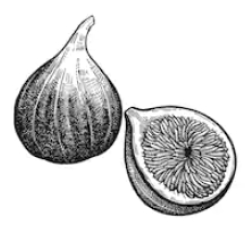
\includegraphics[width=1in,height=1.25in,clip,keepaspectratio]{fig1}}]{Michael Shell}
Use $\backslash${\tt{begin\{IEEEbiography\}}} and then for the 1st argument use $\backslash${\tt{includegraphics}} to declare and link the author photo.
Use the author name as the 3rd argument followed by the biography text.
\end{IEEEbiography}

\vspace{11pt}

\bf{If you will not include a photo:}\vspace{-33pt}
\begin{IEEEbiographynophoto}{John Doe}
Use $\backslash${\tt{begin\{IEEEbiographynophoto\}}} and the author name as the argument followed by the biography text.
\end{IEEEbiographynophoto}




\vfill

\end{document}


